

\subsection{Hiện thực các chức năng cốt lõi và giao diện người dùng}\label{sec:core-function-implementation}

\subsubsection{Xác thực người dùng và phát hành mã QR động}

Người dùng đăng nhập qua \texttt{POST /auth/login} để nhận JWT RS256 lưu trong
\texttt{sessionStorage} (tự xóa khi đóng tab, không dùng refresh token để giảm diện tấn công). Khi
tải trang, giao diện gọi \texttt{GET /auth/me} kiểm tra hiệu lực phiên và vai trò. Nhân viên có vai
trò \texttt{EMPLOYEE} gọi \texttt{GET /portal/qr-token} (không truyền tham số định danh; máy chủ lấy
mã nhân viên trực tiếp từ JWT để ngăn xem hộ mã của người khác theo FR-03). Chuỗi mã QR có định dạng
\texttt{TMC1.<base64url\_payload>.<base64url\_signature>}, hiệu lực 60 giây (chấp nhận lệch đồng hồ
$\pm 30$ giây tại trạm), được đề nghị làm mới mỗi 30 giây và gắn header
\texttt{Cache-Control: no-store}.

Quản trị viên (\texttt{ADMIN}) tra cứu danh sách nhân viên qua \texttt{GET /employees} và thực hiện
cấp mới, cấp lại hoặc thu hồi credential qua \texttt{POST /employees/\{code\}/qr/issue} và
\texttt{POST /employees/\{code\}/qr/revoke}. Khi thu hồi thành công, Portal của nhân viên nhận mã
lỗi \texttt{409 CREDENTIAL\_REVOKED} ở lần làm mới tiếp theo, đồng thời các Gate Agent đang trực
tuyến sẽ cập nhật danh sách từ chối trong vòng tối đa 60 giây. Hình~\ref{fig:ui-login} và
Hình~\ref{fig:ui-portal-qr-states} minh họa kết quả chạy thực tế của màn hình đăng nhập và hai trạng
thái mã QR trên Portal nhân viên.

\begin{figure}[H]
    \centering
    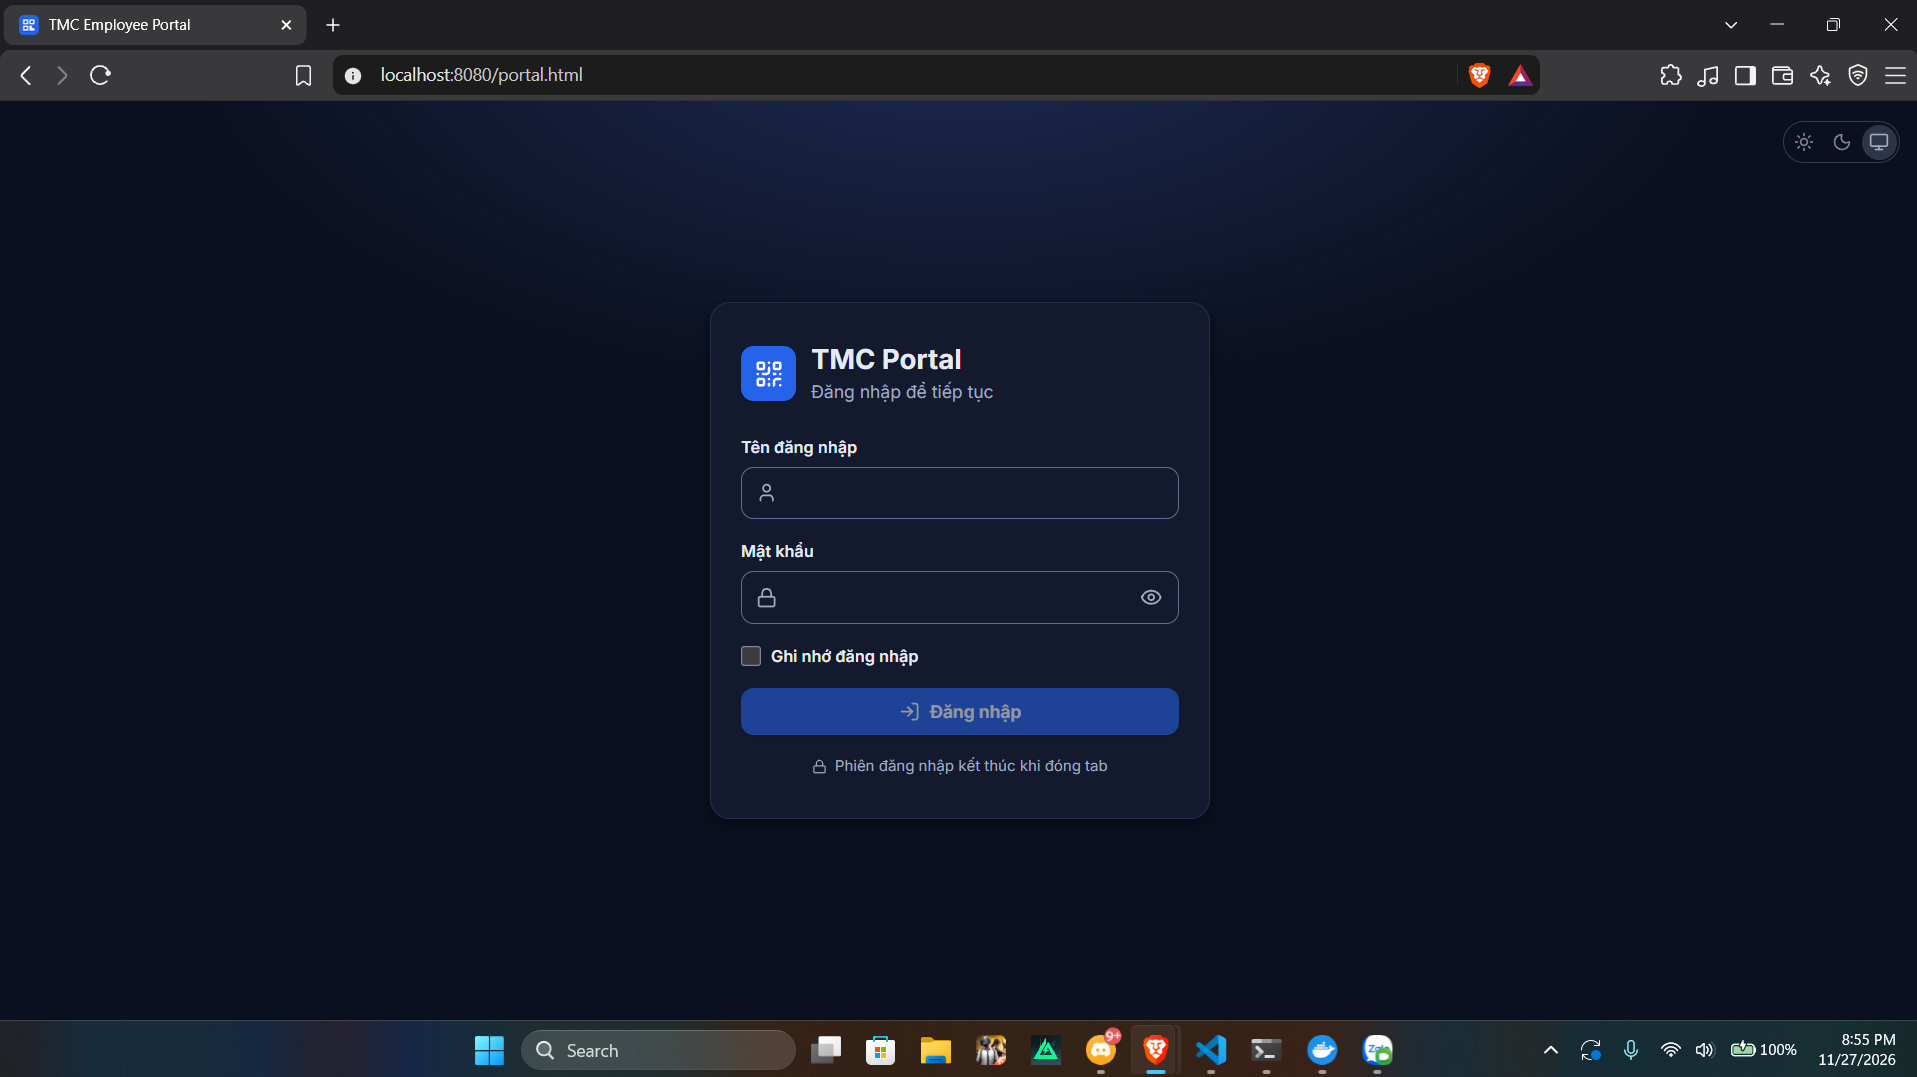
\includegraphics[width=0.82\textwidth]{figures/09_system_implementation/ui_login.png}
    \caption{Giao diện đăng nhập dùng chung cho Portal và Admin (\texttt{AU-01})}
    \label{fig:ui-login}
\end{figure}

\begin{figure}[H]
    \centering
    \begin{subfigure}[b]{0.49\textwidth}
        \centering
        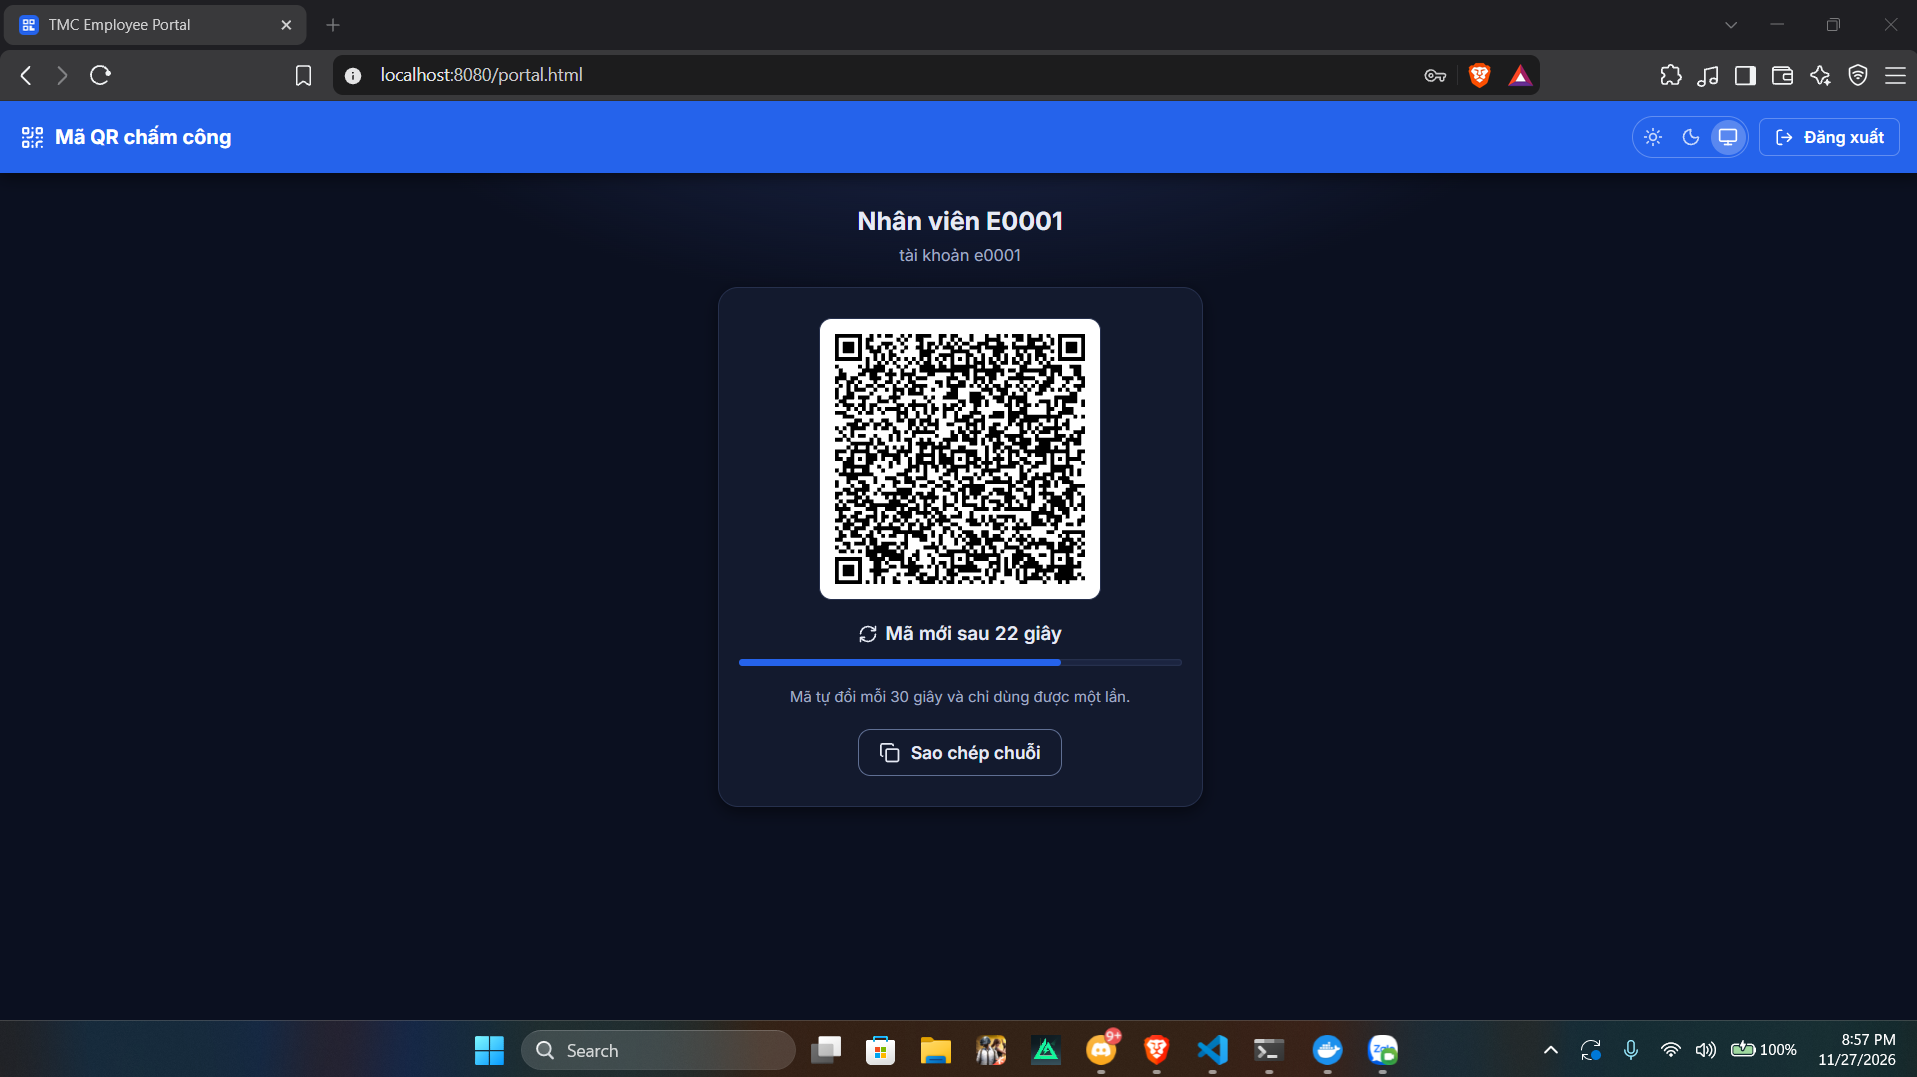
\includegraphics[width=\textwidth]{figures/09_system_implementation/ui_portal_qr.png}
        \caption{Mã QR động của nhân viên \texttt{E0001} (\texttt{P-01})}
        \label{fig:ui-portal-qr}
    \end{subfigure}
    \hfill
    \begin{subfigure}[b]{0.49\textwidth}
        \centering
        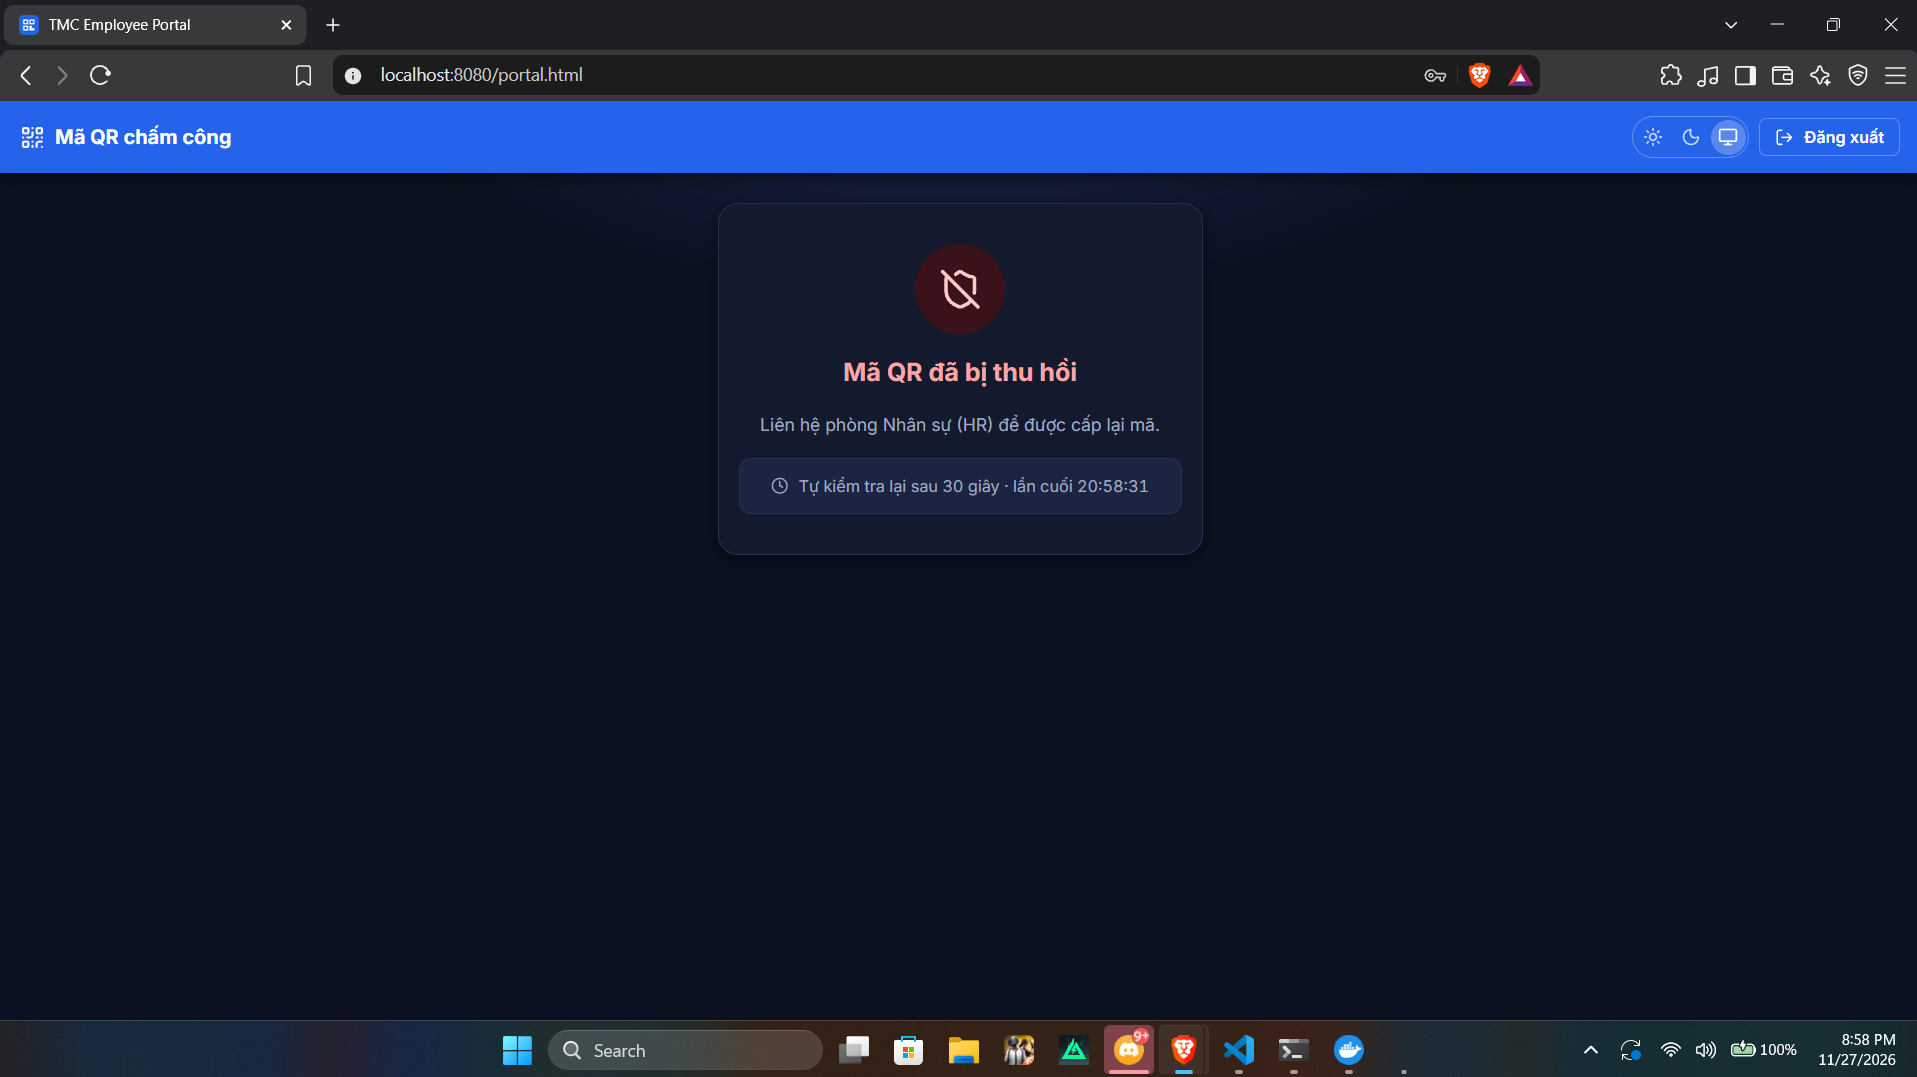
\includegraphics[width=\textwidth]{figures/09_system_implementation/ui_portal_revoked.png}
        \caption{Trạng thái mã QR đã bị thu hồi (\texttt{P-02})}
        \label{fig:ui-portal-revoked}
    \end{subfigure}
    \caption{Kết quả thực thi luồng cấp và thu hồi mã QR động trên Portal nhân viên}
    \label{fig:ui-portal-qr-states}
\end{figure}

\subsubsection{Xử lý lượt quét tại trạm cổng và phân loại kết quả}

Kiosk gửi mã trạm và chuỗi QR quét được tới \texttt{POST /scan} với timeout phía client là 2000 ms,
không tự động thử lại (vì nonce có thể đã bị tiêu thụ) và khóa nhập liệu trong khi đang chờ phản hồi
để tránh quét đúp. Điểm thiết kế quan trọng là mọi kết quả nghiệp vụ đều trả về mã HTTP 200 kèm
trường \texttt{result} thuộc một trong ba giá trị: \texttt{ACCEPTED} (màn hình xanh -- chỉ hiển thị
duy nhất cho trạng thái này theo NFR-AVL-03), \texttt{REJECTED} (màn hình đỏ kèm lý do cụ thể) hoặc
\texttt{GATE\_FAILED} (màn hình cam yêu cầu gặp bảo vệ). Bảng~\ref{tab:scan-reject-reasons} liệt kê
đầy đủ các mã kết quả, lý do từ chối và thông báo tiếng Việt chuẩn hóa giữa Gate Agent và Kiosk.

\small
\begin{longtable}{|>{\raggedright\arraybackslash}p{2.1cm}|>{\raggedright\arraybackslash}p{4.3cm}|>{\raggedright\arraybackslash}p{4.8cm}|>{\raggedright\arraybackslash}p{3.6cm}|}
\caption{Bảng mã kết quả quét, lý do từ chối và thông báo hiển thị trên Kiosk}\label{tab:scan-reject-reasons}\\
\hline
\textbf{Result} & \textbf{Mã \texttt{reason}} & \textbf{Ý nghĩa kỹ thuật} & \textbf{Thông báo Kiosk (Màu)} \\
\hline
\endfirsthead
\hline
\textbf{Result} & \textbf{Mã \texttt{reason}} & \textbf{Ý nghĩa kỹ thuật} & \textbf{Thông báo Kiosk (Màu)} \\
\hline
\endhead
\hline
\multicolumn{4}{r}{\textit{Còn tiếp sang trang sau...}} \\
\hline
\endfoot
\hline
\endlastfoot
\texttt{ACCEPTED} & \textit{(không có)} & Cổng xoay đã xác nhận mở và giao dịch chấm công đã được lưu cục bộ & Mời qua -- \{mã NV\} (VÀO/RA) \textit{(Xanh)} \\
\hline
\texttt{REJECTED} & \texttt{EXPIRED}, \texttt{NOT\_YET\_VALID} & Token ngoài cửa sổ hiệu lực 60 giây ($\pm 30$ giây lệch đồng hồ) & Mã QR đã hết hạn, vui lòng làm mới \textit{(Đỏ)} \\
\hline
\texttt{REJECTED} & \texttt{NONCE\_REUSED} & Token đã được sử dụng trước đó (chống chụp màn hình dùng lại) & Mã QR đã được sử dụng \textit{(Đỏ)} \\
\hline
\texttt{REJECTED} & \texttt{INVALID\_FORMAT}, \texttt{UNKNOWN\_KEY}, \texttt{BAD\_SIGNATURE} & Chuỗi không đúng định dạng \texttt{TMC1.}, khóa không tồn tại hoặc chữ ký sai & Mã QR không hợp lệ \textit{(Đỏ)} \\
\hline
\texttt{REJECTED} & \texttt{CREDENTIAL\_REVOKED}, \texttt{CREDENTIAL\_NOT\_FOUND} & Credential đã bị thu hồi hoặc chưa có trong bản sao cục bộ & Mã QR đã bị thu hồi hoặc không tồn tại \textit{(Đỏ)} \\
\hline
\texttt{REJECTED} & \texttt{EMPLOYEE\_INACTIVE} & Hồ sơ nhân viên không còn hoạt động & Nhân viên không còn hiệu lực \textit{(Đỏ)} \\
\hline
\texttt{REJECTED} & \texttt{UNKNOWN\_STATION}, \texttt{STATION\_DISABLED} & Trạm không thuộc Gate Agent này hoặc đang bị vô hiệu hóa (INV-03) & Trạm đang tạm ngừng \textit{(Đỏ)} \\
\hline
\texttt{REJECTED} & \texttt{ANTI\_PASSBACK} & Quét trùng chiều vào liên tiếp (vi phạm INV-04) & Bạn đã quét vào trước đó \textit{(Đỏ)} \\
\hline
\texttt{REJECTED} & \texttt{OFFLINE\_THRESHOLD\_EXCEEDED} & Cổng chiều vào bị từ chối do mất kết nối WAN vượt ngưỡng cho phép & Mất kết nối quá lâu -- vui lòng gặp bảo vệ \textit{(Đỏ)} \\
\hline
\texttt{GATE\_FAILED} & \texttt{GATE\_TIMEOUT}, \texttt{GATE\_ERROR}, \texttt{CIRCUIT\_OPEN} & Luật hợp lệ nhưng cổng xoay quá 800 ms, báo lỗi hoặc đang ngắt mạch 30 giây & Cổng chưa mở -- vui lòng gặp bảo vệ \textit{(Cam)} \\
\hline
\textit{Lỗi kết nối / HTTP 5xx} & \textit{(timeout client $> 2$ s)} & Không nhận được phản hồi xác định từ Gate Agent & Không xác định -- vui lòng gặp bảo vệ \textit{(Cam)} \\
\hline
\end{longtable}
\normalsize

Hình~\ref{fig:ui-kiosk-scan-results} minh họa hai kết quả thực thi thực tế tại trạm \texttt{BD-IN-01}:
lượt quét hợp lệ của nhân viên \texttt{E0001} được chấp nhận và mở cổng trong \textbf{0,37 giây}
(đáp ứng NFR-PER-01 $\leq 2$ giây), và lượt quét vào lặp lại ngay sau đó bị từ chối với lỗi chống
quét trùng làn (\texttt{ANTI\_PASSBACK}, INV-04) trong \textbf{0,01 giây}.

\begin{figure}[H]
    \centering
    \begin{subfigure}[b]{0.49\textwidth}
        \centering
        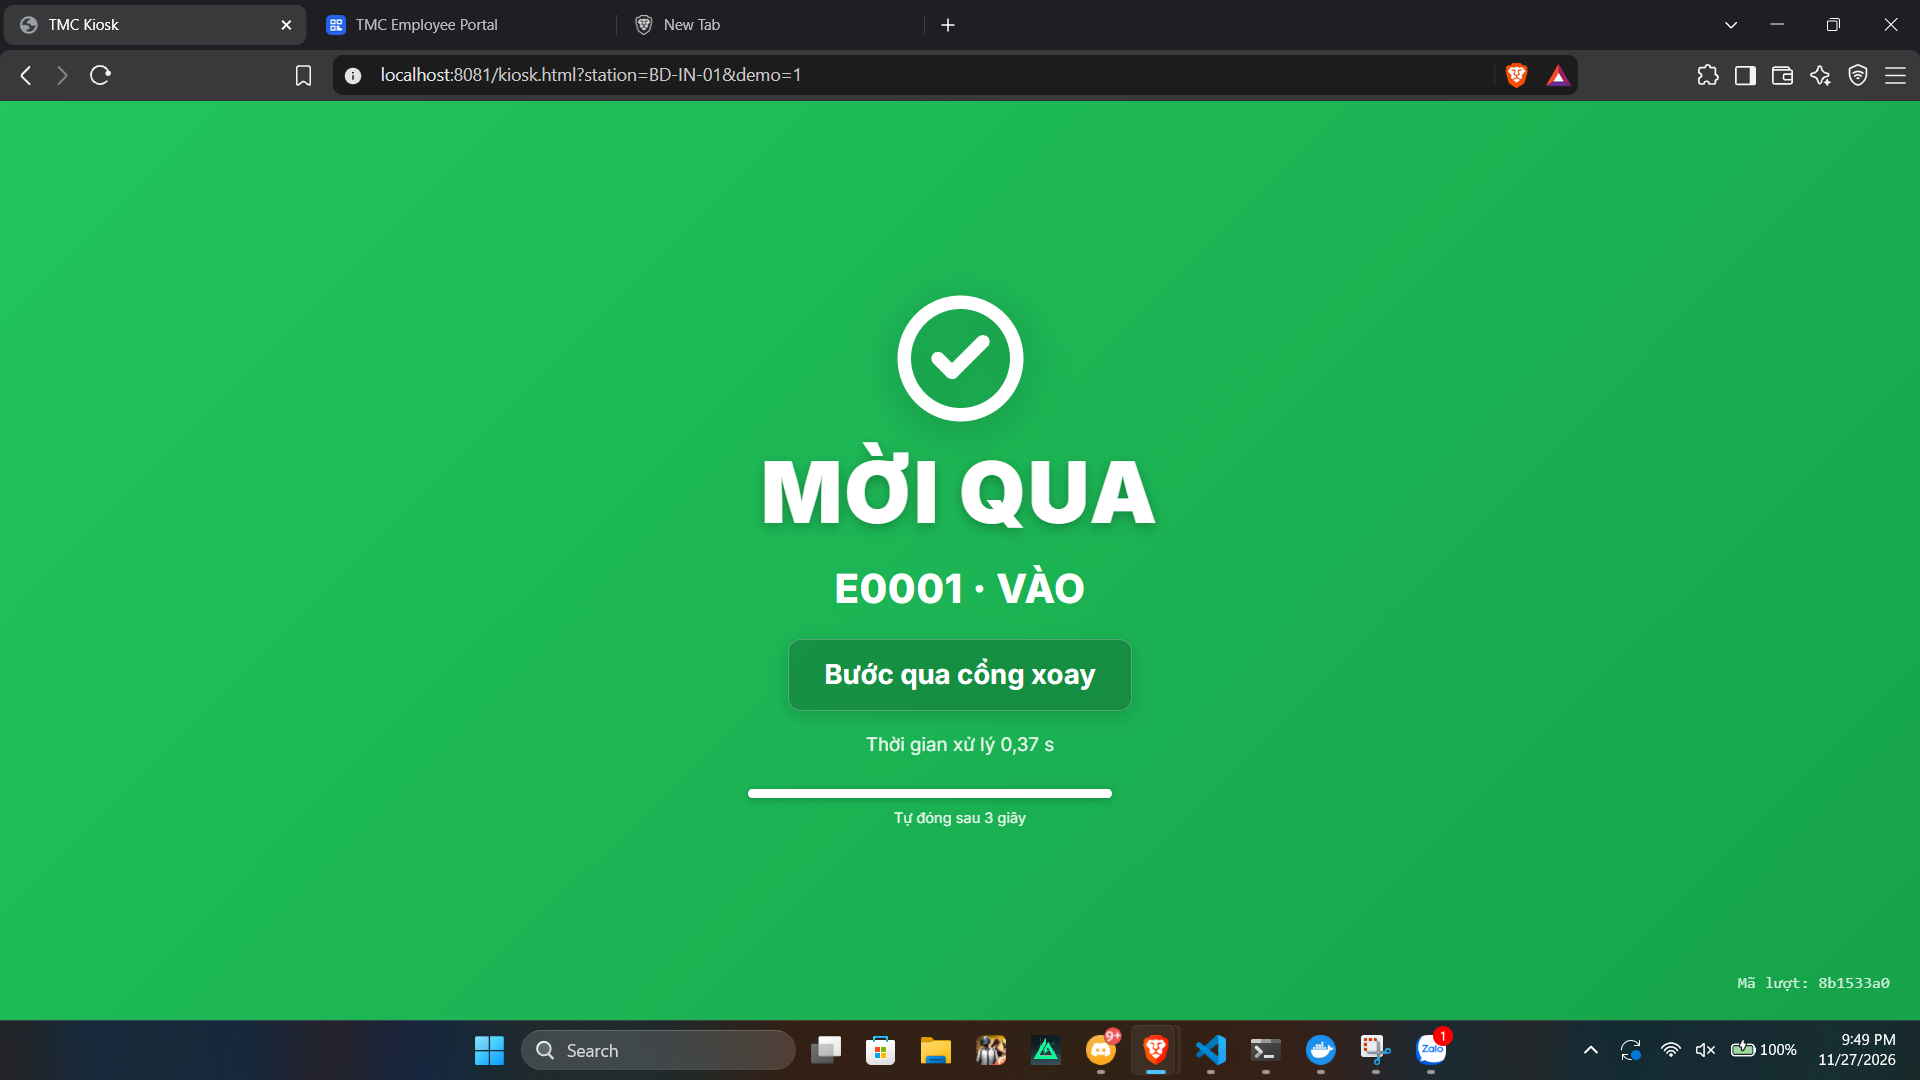
\includegraphics[width=\textwidth]{figures/09_system_implementation/ui_kiosk_accepted.png}
        \caption{Chấp nhận và mở cổng (\texttt{ACCEPTED}, 0,37 s)}
        \label{fig:ui-kiosk-accepted}
    \end{subfigure}
    \hfill
    \begin{subfigure}[b]{0.49\textwidth}
        \centering
        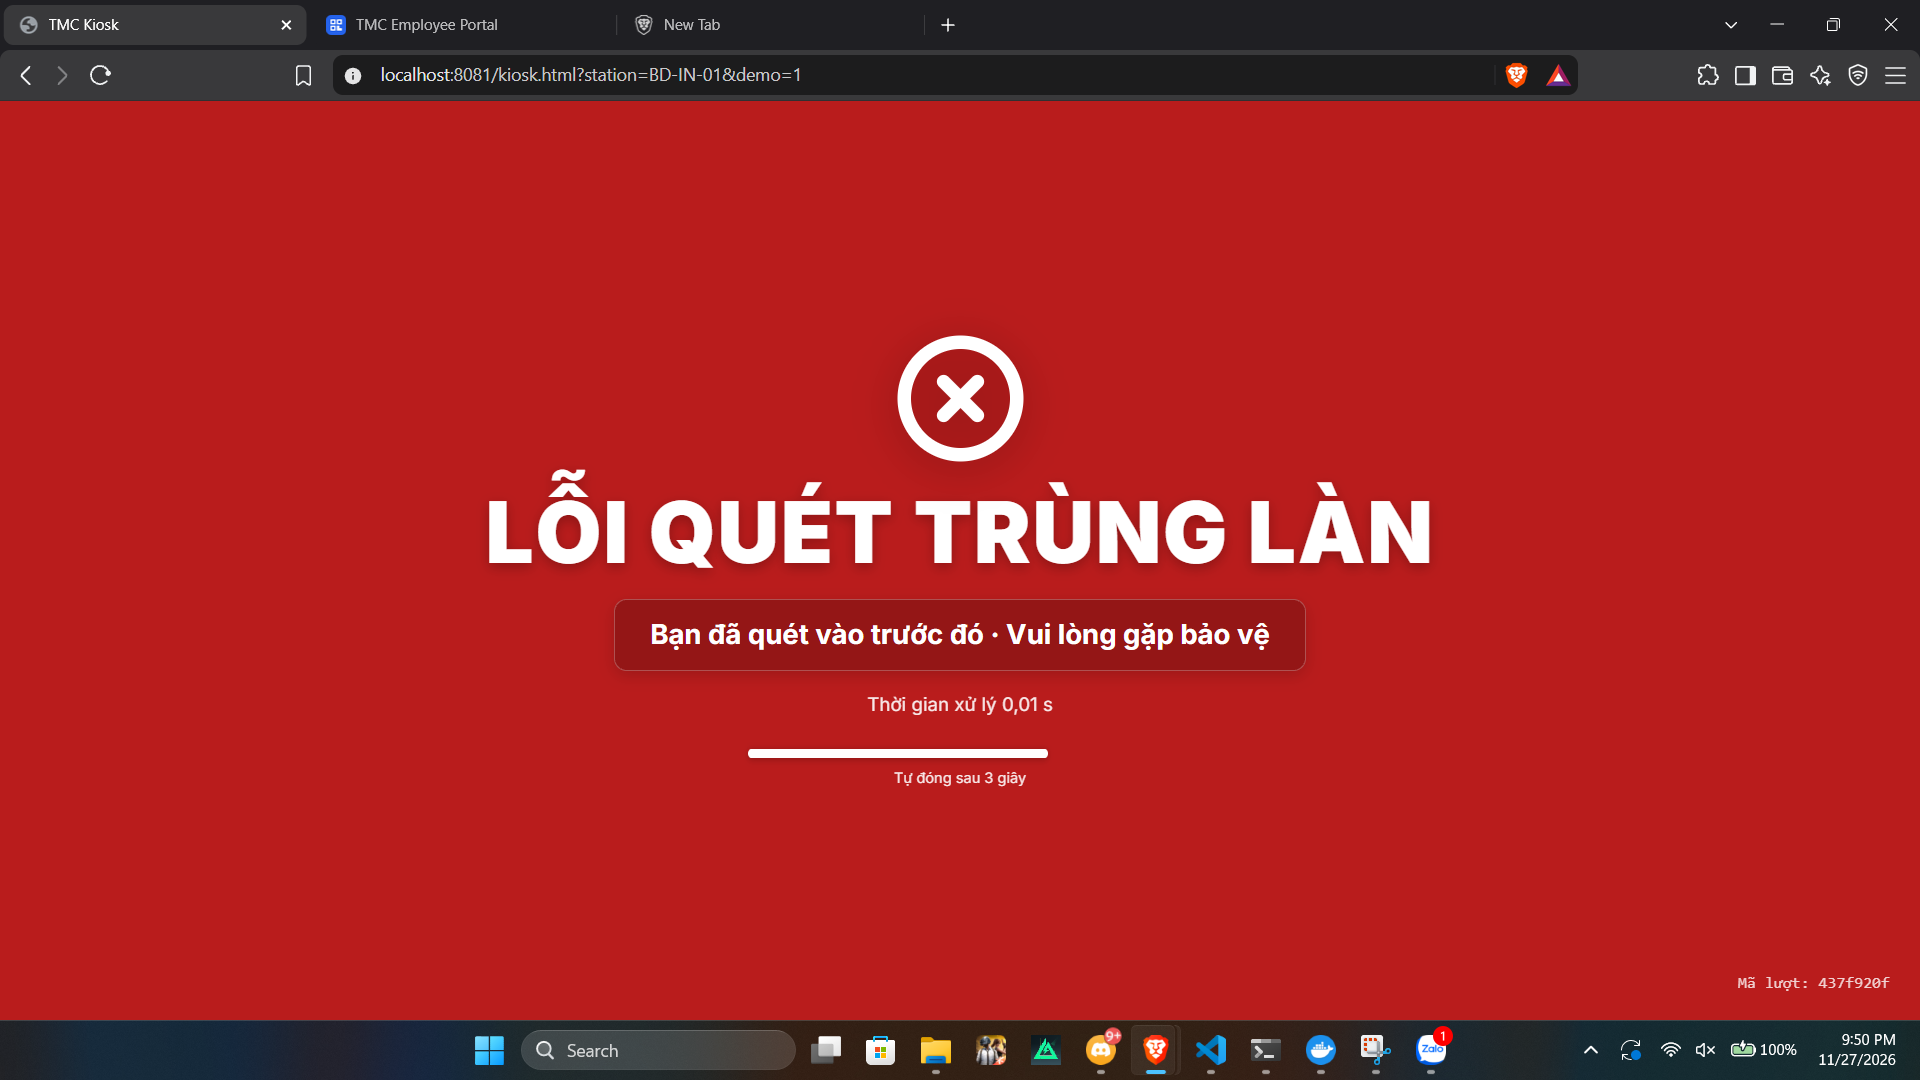
\includegraphics[width=\textwidth]{figures/09_system_implementation/ui_kiosk_rejected.png}
        \caption{Từ chối trùng làn (\texttt{ANTI\_PASSBACK}, 0,01 s)}
        \label{fig:ui-kiosk-rejected}
    \end{subfigure}
    \caption{Kết quả hiển thị màn hình phủ \texttt{K-02} tại trạm cổng \texttt{BD-IN-01}}
    \label{fig:ui-kiosk-scan-results}
\end{figure}

\subsubsection{Lưu trữ cục bộ, hoạt động ngoại tuyến và giả lập cổng xoay}

Khi kết nối WAN tới Central bị gián đoạn (không có trao đổi thành công trong 30 giây), Gate Agent
chuyển sang trạng thái ngoại tuyến: mọi lượt quét tiếp tục được xác thực bằng dữ liệu tham chiếu
trong SQLite và lưu vào outbox để gửi bù khi có mạng. Nhằm cân bằng giữa tính sẵn sàng và bảo mật,
chiều \texttt{OUT} luôn tiếp tục hoạt động để không giữ nhân viên trong nhà máy, còn chiều
\texttt{IN} sẽ bị từ chối với lý do \texttt{OFFLINE\_THRESHOLD\_EXCEEDED} nếu thời gian mất kết nối
vượt ngưỡng cấu hình (mặc định 8 giờ trong vận hành và 2 phút trong cấu hình trình diễn). Kiosk định
kỳ gọi \texttt{GET /status} mỗi 3 giây để hiển thị biểu ngữ cảnh báo \textit{``OFFLINE -- \{n\} bản
ghi chờ đồng bộ''} và thông báo tạm ngừng chiều vào khi vượt ngưỡng.

Ở phía thiết bị, dịch vụ \texttt{turnstile-sim} mô phỏng chính xác API nhà cung cấp cổng xoay với
bốn chế độ điều khiển động qua \texttt{PUT /admin/behavior}:
\begin{itemize}
    \item \texttt{NORMAL}: mở cổng sau độ trễ ngẫu nhiên trong khoảng \texttt{latencyMs} (mặc định
    300--500 ms) và có thể phát sinh lỗi HTTP 500 theo xác suất \texttt{failureRate}.
    \item \texttt{TIMEOUT}: không mở cổng và trì hoãn 5 giây trước khi trả HTTP 504 (kích hoạt
    timeout 800 ms của Gate Agent).
    \item \texttt{ERROR}: không mở cổng và trả ngay HTTP 500 (\texttt{SIMULATED\_ERROR}).
    \item \texttt{EXECUTE\_THEN\_TIMEOUT}: vẫn thực thi mở cổng nhưng trì hoãn phản hồi 5 giây, dùng
    để kiểm chứng cơ chế truy vấn đối soát lệnh \texttt{GET /turnstiles/\{id\}/commands/\{requestId\}}
    của Gate Agent.
\end{itemize}

Hình~\ref{fig:ui-kiosk-outbox-sync} minh họa màn hình chờ quét làn vào (\texttt{K-01}) kết hợp bảng
điều khiển demo (\texttt{K-05}) khi Gate Agent đang đẩy bù các bản ghi còn tồn trong hàng đợi outbox
về Central sau khi khôi phục kết nối.

\begin{figure}[H]
    \centering
    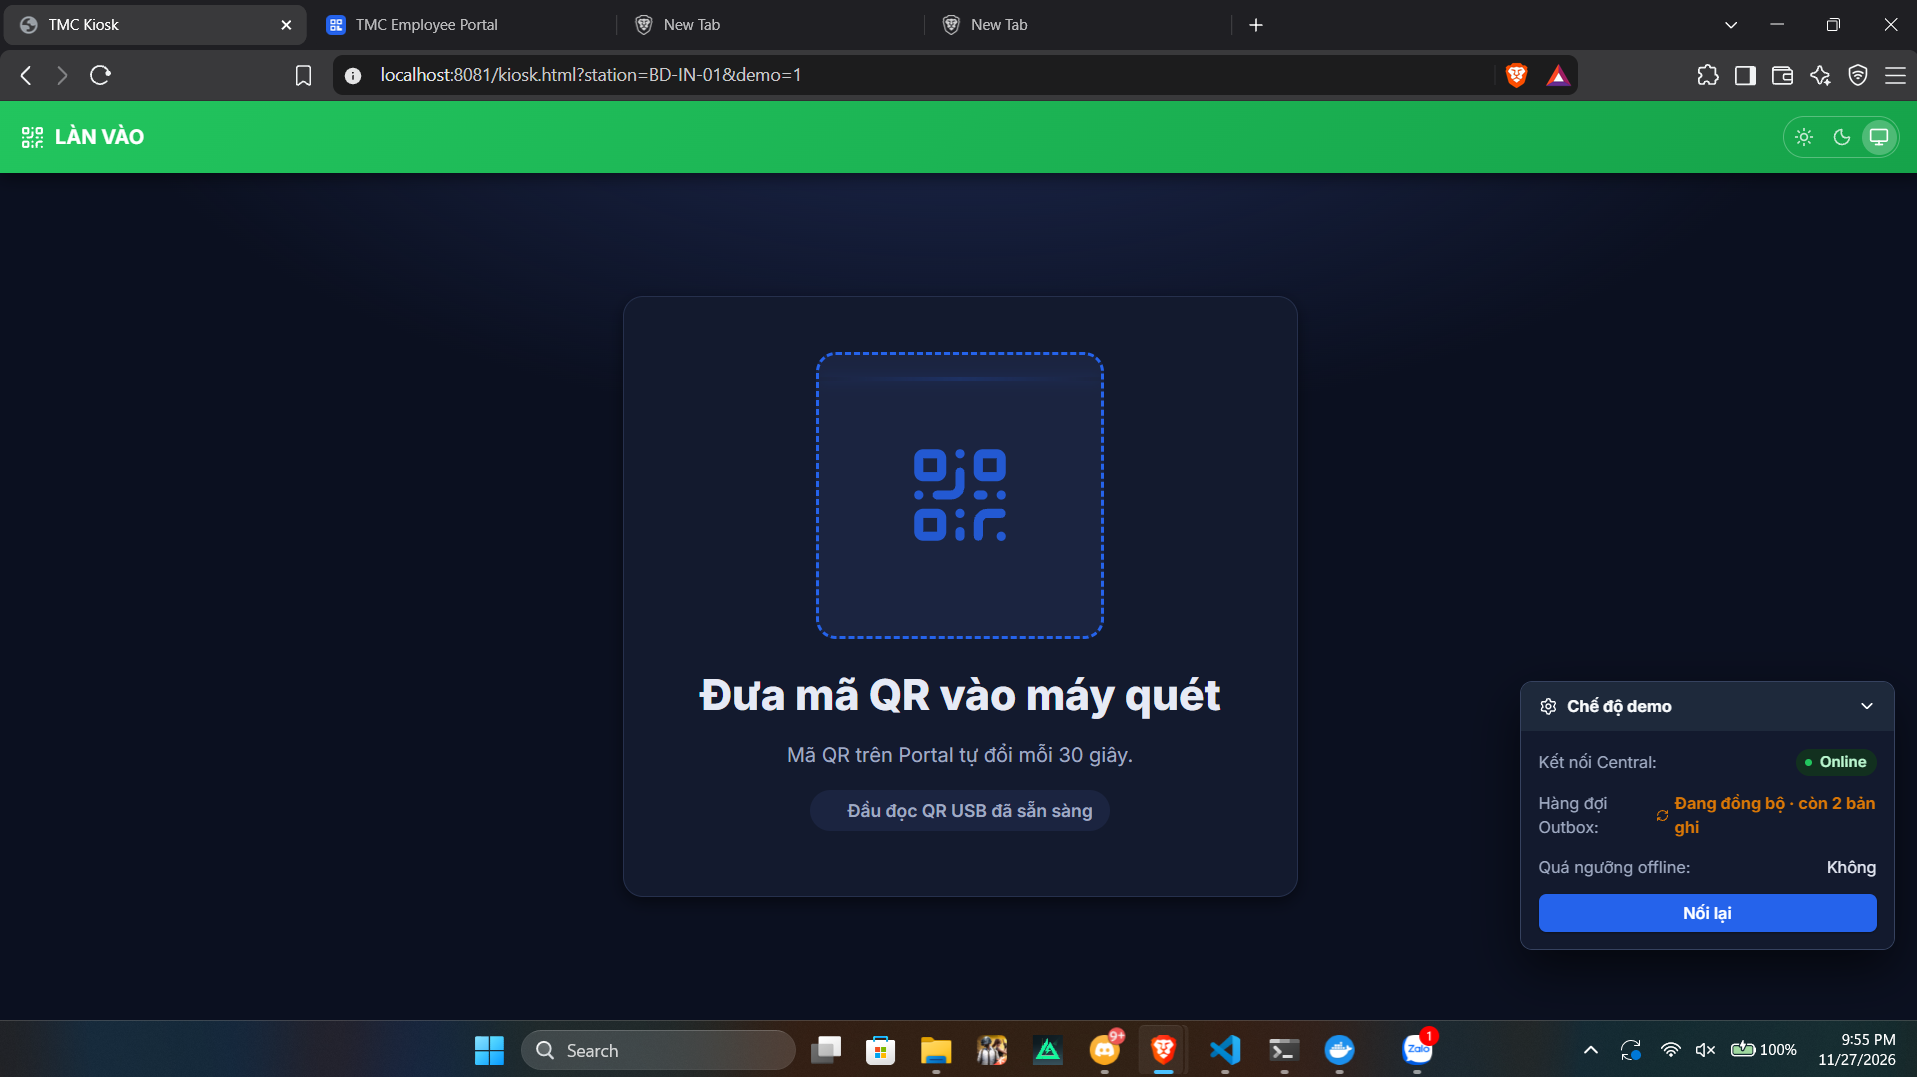
\includegraphics[width=0.82\textwidth]{figures/09_system_implementation/ui_kiosk_offline.png}
    \caption{Màn hình Kiosk làn vào (\texttt{K-01}) kèm bảng điều khiển demo (\texttt{K-05}) hiển thị hàng đợi outbox đang đồng bộ bù}
    \label{fig:ui-kiosk-outbox-sync}
\end{figure}

\subsubsection{Kiến trúc giao diện web và danh mục màn hình (Sitemap)}

Giao diện web được xây dựng bằng React và TypeScript, tách thành hai gói biên dịch độc lập: gói
\texttt{gate} (chỉ chứa trang \texttt{kiosk.html}, nhúng trực tiếp vào Gate Agent) và gói
\texttt{central} (chứa hai trang \texttt{portal.html} và \texttt{admin.html}, nhúng trực tiếp vào
Central). Cách đóng gói cùng nguồn gốc (same-origin) loại bỏ nhu cầu cấu hình CORS. Riêng trang
\texttt{admin.html} sử dụng định tuyến dạng hash (\texttt{\#/employees}, \texttt{\#/stations}) để
máy chủ tĩnh phục vụ trực tiếp mà không cần luật fallback SPA.

Về cấu trúc mã nguồn frontend, các thành phần được chia thành bốn lớp rõ ràng: lớp khởi tạo trang
(\texttt{entries}), lớp tính năng theo nghiệp vụ (\texttt{features/kiosk}, \texttt{features/portal},
\texttt{features/admin}, \texttt{features/auth}), lớp giao tiếp API dùng chung
(\texttt{shared/api/gateApi}, \texttt{shared/api/centralApi}, \texttt{shared/api/authSession} -- là
nơi duy nhất được phép gọi HTTP, sử dụng kiểu TypeScript sinh tự động từ OpenAPI 3.0.3) và lớp thành
phần hiển thị/hook dùng chung (\texttt{shared/ui}, \texttt{shared/hooks}).

Toàn bộ sitemap của phiên bản MVP gồm 14 màn hình, trạng thái và thành phần tương tác được đặc tả đầy
đủ trong Bảng~\ref{tab:web-sitemap-catalog}.

\small
\begin{longtable}{|>{\raggedright\arraybackslash}p{1.2cm}|>{\raggedright\arraybackslash}p{2.4cm}|>{\raggedright\arraybackslash}p{2.4cm}|>{\raggedright\arraybackslash}p{3.0cm}|>{\raggedright\arraybackslash}p{5.6cm}|}
\caption{Danh mục đầy đủ 14 màn hình và trạng thái giao diện web của MVP}\label{tab:web-sitemap-catalog}\\
\hline
\textbf{Mã} & \textbf{Tên màn hình} & \textbf{Trang / Loại} & \textbf{API sử dụng} & \textbf{Chức năng và hành vi chính} \\
\hline
\endfirsthead
\hline
\textbf{Mã} & \textbf{Tên màn hình} & \textbf{Trang / Loại} & \textbf{API sử dụng} & \textbf{Chức năng và hành vi chính} \\
\hline
\endhead
\hline
\multicolumn{5}{r}{\textit{Còn tiếp sang trang sau...}} \\
\hline
\endfoot
\hline
\endlastfoot
\texttt{K-01} & Chờ quét & \texttt{kiosk.html} \textit{(screen)} & \texttt{GET /status}, \texttt{POST /scan} & Màn hình chính tại trạm cổng (\texttt{?station=<id>}); giữ tiêu điểm (focus) trên ô nhập ẩn để nhận chuỗi từ máy quét USB; hiển thị biểu ngữ trạng thái mạng và độ sâu outbox mỗi 3 giây. \\
\hline
\texttt{K-02} & Kết quả quét & Phủ lên \texttt{K-01} \textit{(overlay)} & Kết quả \texttt{POST /scan} & Hiển thị nền xanh (\texttt{ACCEPTED}), đỏ (\texttt{REJECTED}) hoặc cam (\texttt{GATE\_FAILED}) kèm mã nhân viên, chiều vào/ra, thời gian xử lý (\texttt{elapsedMs}); tự đóng về \texttt{K-01} sau 3 giây. \\
\hline
\texttt{K-03} & Lỗi cấu hình trạm & \texttt{kiosk.html} \textit{(screen)} & \texttt{GET /status} & Hiển thị cho kỹ thuật viên khi thiếu tham số \texttt{station} hoặc mã trạm không thuộc danh sách trạm của Gate Agent. \\
\hline
\texttt{K-04} & Quét bằng webcam & \texttt{?camera=1} \textit{(mode)} & \texttt{POST /scan} & Bổ sung khung camera trực tiếp trên \texttt{K-01} để giải mã QR bằng webcam khi không có đầu đọc USB. \\
\hline
\texttt{K-05} & Bảng điều khiển demo & \texttt{?demo=1} \textit{(panel)} & \texttt{POST} \path{/admin/simulate-offline}, \texttt{GET /status} & Bảng bật/tắt giả lập mất kết nối WAN và theo dõi thông số outbox trực tiếp trên kiosk trong cấu hình demo. \\
\hline
\texttt{AU-01} & Đăng nhập & \texttt{portal.html}, \texttt{admin.html} \textit{(screen)} & \texttt{POST /auth/login}, \texttt{GET /auth/me} & Biểu mẫu nhập tài khoản/mật khẩu dùng chung cho Portal và Admin; khóa nút gửi khi đang xử lý; lưu JWT vào \texttt{sessionStorage}. \\
\hline
\texttt{AU-02} & Không có quyền truy cập & \texttt{portal.html}, \texttt{admin.html} \textit{(screen)} & \texttt{GET /auth/me} & Hiển thị khi tài khoản đã đăng nhập hợp lệ nhưng sai vai trò trang (ví dụ \texttt{ADMIN} mở Portal hoặc \texttt{EMPLOYEE} mở Admin), kèm nút đăng xuất. \\
\hline
\texttt{P-01} & Mã QR cá nhân & \texttt{portal.html} \textit{(screen)} & \texttt{GET} \path{/portal/qr-token} & Hiển thị mã QR động (mức sửa lỗi M) kèm đồng hồ đếm ngược 60 giây (tự động bù lệch đồng hồ máy chủ qua header \texttt{Date}); làm mới mỗi 30 giây và khi mở lại tab; có nút sao chép chuỗi QR. \\
\hline
\texttt{P-02} & Không có mã QR & \texttt{portal.html} \textit{(state)} & \texttt{GET} \path{/portal/qr-token} (409) & Thay thế \texttt{P-01} khi mã đã bị thu hồi, chưa được cấp hoặc nhân viên ngừng hoạt động; tự động hỏi lại mỗi 30 giây để hiển thị ngay khi HR cấp lại. \\
\hline
\texttt{A-01} & Khung trang quản trị & \texttt{admin.html} \textit{(layout)} & \texttt{GET /auth/me} & Thanh điều hướng chứa tên tài khoản, nút đăng xuất và hai tab chuyển đổi giữa \texttt{A-02} (\texttt{\#/employees}) và \texttt{A-04} (\texttt{\#/stations}). \\
\hline
\texttt{A-02} & Tab Nhân viên & \texttt{\#/employees} \textit{(tab)} & \texttt{GET /employees} & Bảng danh sách nhân viên kèm trạng thái credential; hỗ trợ lọc theo phòng ban, tìm kiếm theo mã/tên (debounce 300 ms), chọn từng dòng hoặc nhiều dòng. \\
\hline
\texttt{A-03} & Hộp thoại thao tác QR & Dialog trên \texttt{A-02} & \texttt{POST} \path{.../qr/revoke}, \texttt{POST} \path{.../qr/issue} & Xác nhận cấp lại hoặc thu hồi mã QR cho một nhân viên; bắt buộc nhập lý do (3--200 ký tự) khi thu hồi và cập nhật lại đúng dòng nhân viên sau khi hoàn tất. \\
\hline
\texttt{A-04} & Tab Trạm & \texttt{\#/stations} \textit{(tab)} & \texttt{GET /stations} & Theo dõi danh sách trạm cổng của hai nhà máy, làm mới mỗi 5 giây: trạng thái trực tuyến/ngoại tuyến, thời điểm heartbeat gần nhất, độ sâu outbox và trạng thái cổng xoay. \\
\hline
\texttt{A-05} & Hộp thoại thao tác hàng loạt & Dialog trên \texttt{A-02} & \texttt{POST} \path{.../qr/revoke}, \texttt{POST} \path{.../qr/issue} & Hỗ trợ thu hồi hoặc cấp lại mã QR cho nhiều nhân viên đã chọn bằng cách gọi tuần tự từng API, kiểm tra điều kiện trước khi chạy, yêu cầu nhập chuỗi xác nhận nếu thu hồi từ 5 người trở lên và dừng ngay khi gặp 401/403. \\
\hline
\end{longtable}
\normalsize

Quy tắc bảo vệ điều hướng (route guard) của Portal và Admin được thực thi nhất quán: khi mở trang,
nếu không có token trong \texttt{sessionStorage} hoặc \texttt{GET /auth/me} trả về 401 thì xóa phiên
và chuyển về \texttt{AU-01}; nếu trả về 200 nhưng vai trò không khớp trang thì chuyển sang
\texttt{AU-02}. Mọi thao tác bị từ chối 401 từ bất kỳ màn hình nào đều buộc đăng nhập lại. Riêng
Kiosk (\texttt{K-01}--\texttt{K-05}) hoạt động không cần đăng nhập trong mạng LAN cô lập của nhà máy
theo ADR-08. Hình~\ref{fig:ui-admin-employees} và Hình~\ref{fig:ui-admin-stations} minh họa giao diện
quản trị thực tế của hai tab Nhân viên và Trạm cổng.

\begin{figure}[H]
    \centering
    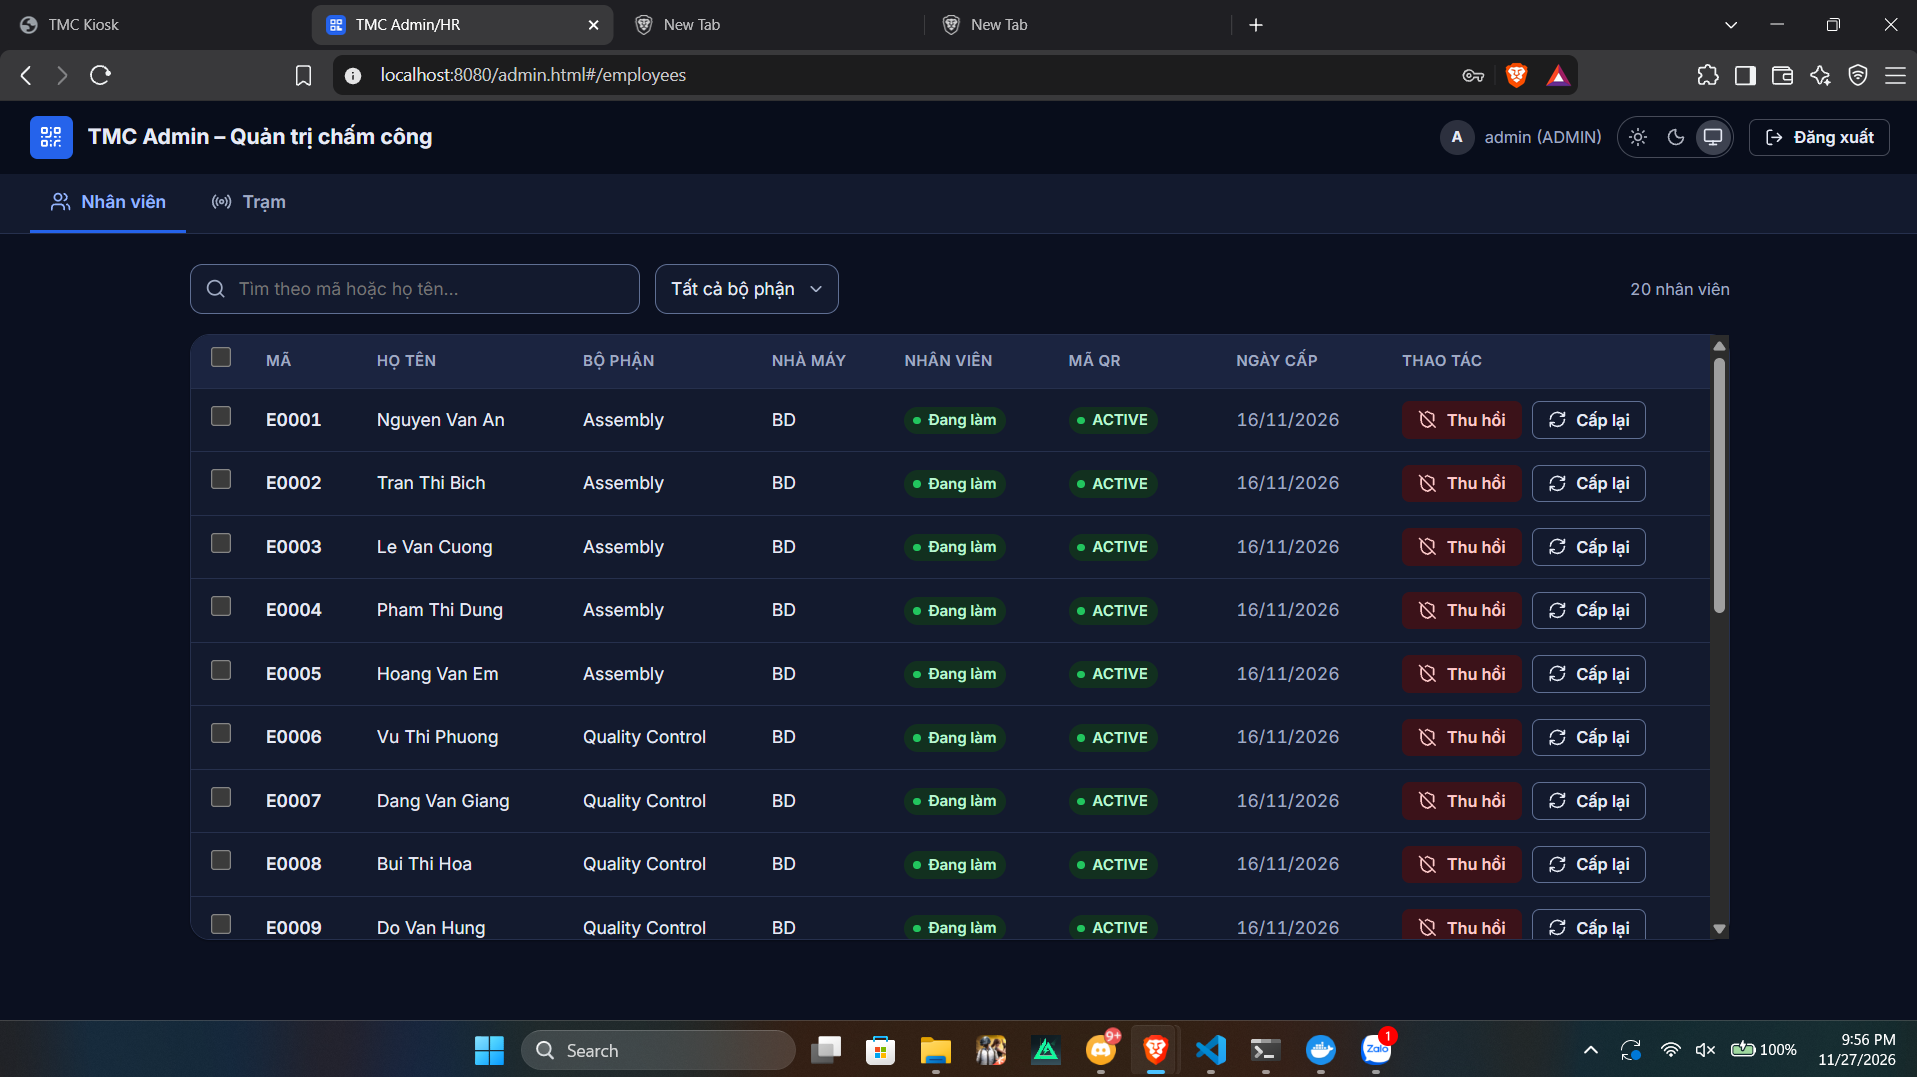
\includegraphics[width=0.88\textwidth]{figures/09_system_implementation/ui_admin_employees.png}
    \caption{Giao diện quản trị tab Nhân viên (\texttt{A-02}) hỗ trợ tìm kiếm, lọc bộ phận và thao tác cấp lại/thu hồi mã QR}
    \label{fig:ui-admin-employees}
\end{figure}

\begin{figure}[H]
    \centering
    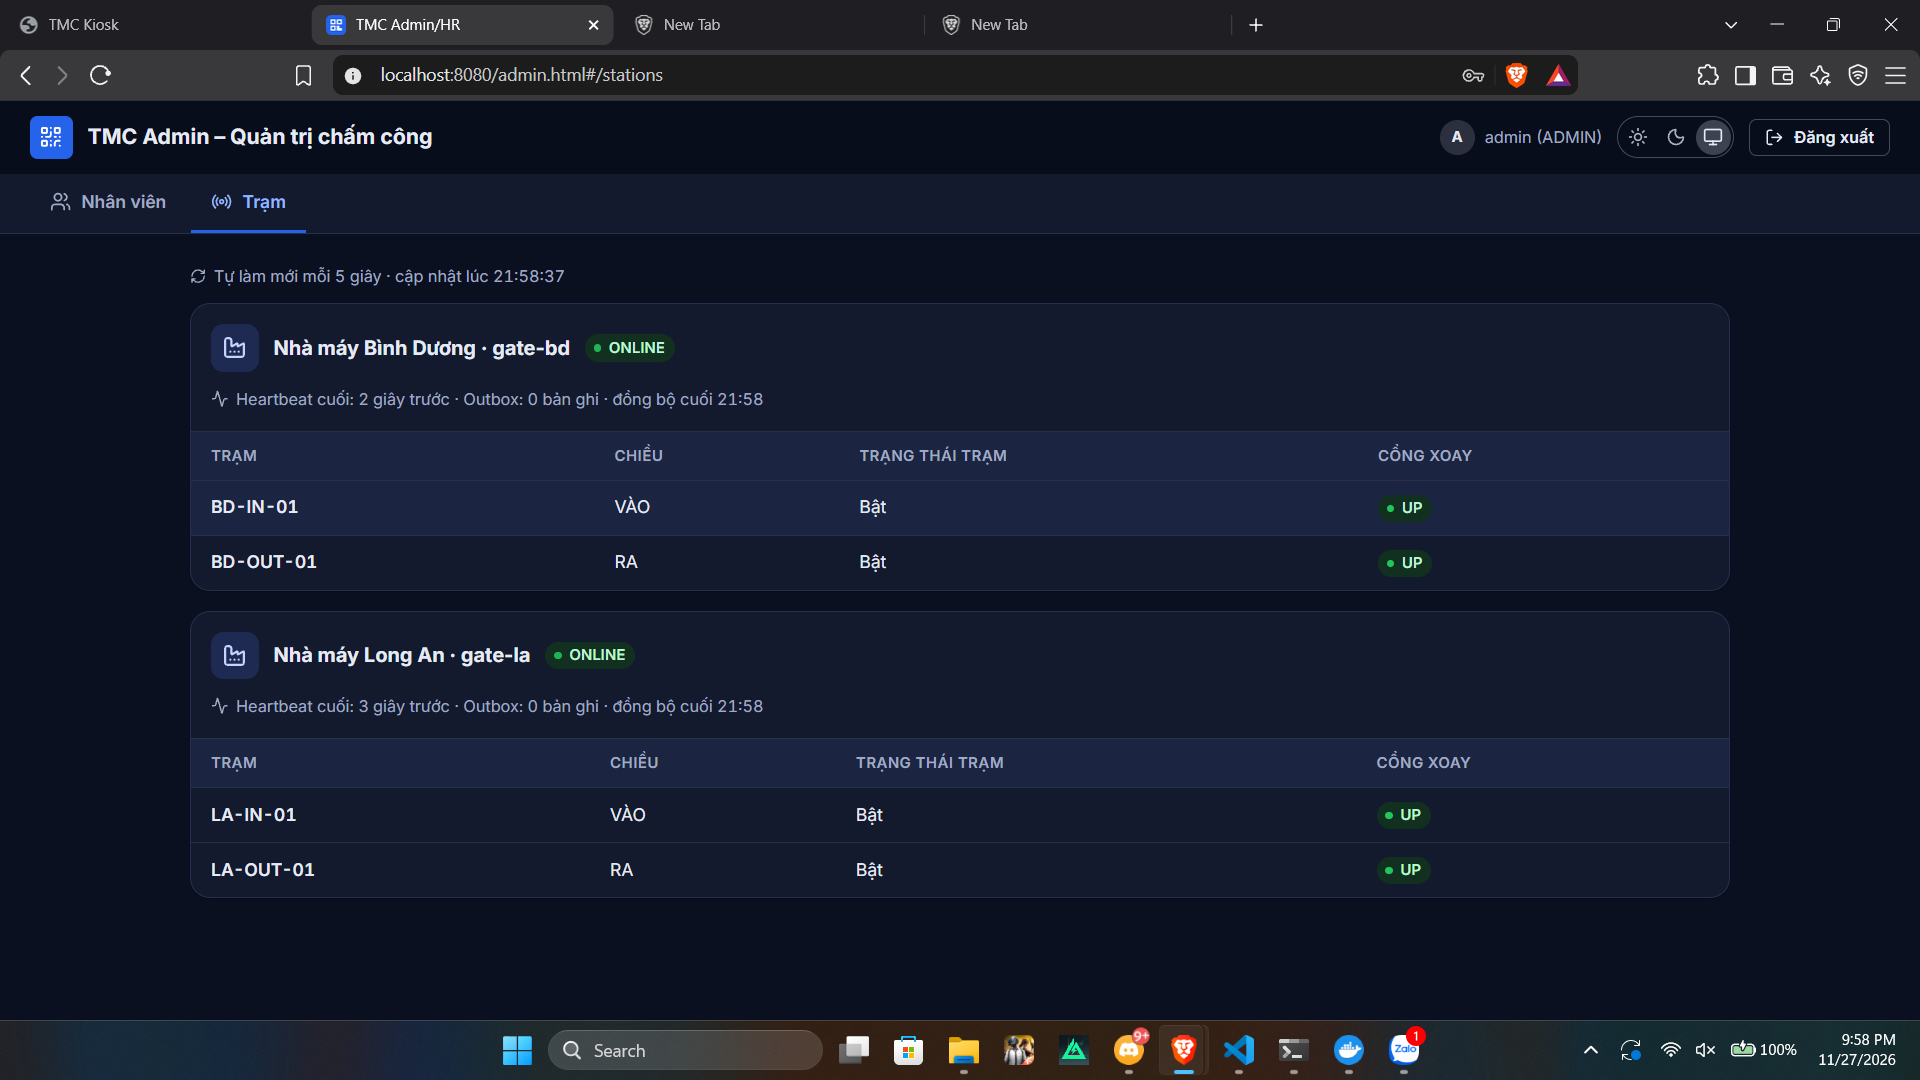
\includegraphics[width=0.88\textwidth]{figures/09_system_implementation/ui_admin_stations.png}
    \caption{Giao diện quản trị tab Trạm (\texttt{A-04}) giám sát trạng thái trực tuyến, heartbeat, outbox và cổng xoay của hai nhà máy}
    \label{fig:ui-admin-stations}
\end{figure}

\subsection{Thiết kế và đặc tả hợp đồng API}\label{sec:api-design-implementation}

\subsubsection{Phương pháp contract-first và quy ước chung}

Hệ thống áp dụng phương pháp thiết kế API theo hướng \textit{contract-first} bằng đặc tả OpenAPI
3.0.3, làm chuẩn thống nhất cho cả sinh mã kiểu TypeScript phía frontend, tạo dữ liệu giả lập MSW và
đối chiếu tài liệu runtime tại \texttt{/v3/api-docs} do Springdoc công bố. Các quy ước giao tiếp dùng
chung trên toàn bộ 19 đường dẫn (20 thao tác) gồm:
\begin{itemize}
    \item \textbf{Định dạng dữ liệu:} Request và response thành công dùng
    \texttt{application/json; charset=utf-8} với tên trường theo \texttt{camelCase}, giá trị enum
    theo \texttt{UPPER\_SNAKE\_CASE}, dấu thời gian theo chuẩn ISO-8601 UTC (hậu tố \texttt{Z}), mã
    sự kiện và credential theo UUID v4, mã nhân viên theo mẫu \texttt{E[0-9]\{4\}}, mã trạm theo mẫu
    \texttt{[A-Z]\{2\}-(IN|OUT)-[0-9]\{2\}}.
    \item \textbf{Tương thích ngược:} Các trường không có giá trị được lược bỏ thay vì trả
    \texttt{null}; cả client và server đều bỏ qua trường chưa biết để việc bổ sung trường tùy chọn
    không phá vỡ các phiên bản đang chạy.
    \item \textbf{Định dạng lỗi chuẩn:} Mọi lỗi giao thức trả về theo chuẩn RFC 9457 Problem Details
    (media type \path{application/problem+json}) gồm \texttt{type}, \texttt{title}, \texttt{status},
    \texttt{detail} và trường \texttt{code} ổn định để client rẽ nhánh xử lý (riêng mã
    \texttt{VALIDATION\_ERROR} kèm thêm mảng \texttt{errors: [\{field, message\}]}).
    \item \textbf{Bảo mật nhật ký:} Tuyệt đối không ghi chuỗi QR thô (\texttt{raw}), JWT, mật khẩu
    hay \texttt{X-Gate-Key} vào log ứng dụng; chỉ ghi \texttt{eventId}, \texttt{cid} và tên đăng nhập
    (NFR-PRI-03).
\end{itemize}

\subsubsection{Danh mục đầy đủ các endpoint}

Hợp đồng API được chia thành bốn nhóm tương ứng với từng ranh giới triển khai và đối tượng tiêu thụ:
\textbf{Gate Agent} (cổng \texttt{:8081}/\texttt{:8082}, phục vụ Kiosk và bảo vệ), \textbf{Central}
(cổng \texttt{:8080}, phục vụ Portal và Admin), \textbf{Sync} (cổng \texttt{:8080/sync}, kết nối giữa
hai quantum Q1--Q2) và \textbf{Turnstile Simulator} (cổng \texttt{:9001}/\texttt{:9002}, giả lập
thiết bị cổng xoay). Bảng~\ref{tab:mvp-api-index} liệt kê toàn bộ 19 path / 20 operation của MVP.

\small
\begin{longtable}{|>{\raggedright\arraybackslash}p{1.9cm}|>{\raggedright\arraybackslash}p{1.5cm}|>{\raggedright\arraybackslash}p{4.6cm}|>{\raggedright\arraybackslash}p{2.2cm}|>{\raggedright\arraybackslash}p{4.4cm}|}
\caption{Danh mục đầy đủ 19 đường dẫn (20 thao tác) API của phiên bản MVP}\label{tab:mvp-api-index}\\
\hline
\textbf{Nhóm} & \textbf{Method} & \textbf{Path} & \textbf{Xác thực} & \textbf{Chức năng} \\
\hline
\endfirsthead
\hline
\textbf{Nhóm} & \textbf{Method} & \textbf{Path} & \textbf{Xác thực} & \textbf{Chức năng} \\
\hline
\endhead
\hline
\multicolumn{5}{r}{\textit{Còn tiếp sang trang sau...}} \\
\hline
\endfoot
\hline
\endlastfoot
Gate Agent & POST & \path{/scan} & LAN (không) & Xác minh QR, ghi lượt quét và mở cổng xoay \\
\hline
Gate Agent & GET & \path{/status} & LAN (không) & Trạng thái kết nối, outbox và sức khỏe cổng \\
\hline
Gate Agent & GET & \path{/guard/pending} & LAN (không) & Danh sách lượt còn \texttt{PENDING} trước khi khởi động lại \\
\hline
Gate Agent & POST & \path{/admin/simulate-offline} & LAN (profile demo) & Bật/tắt giả lập mất kết nối WAN \\
\hline
Central & POST & \path{/auth/login} & Công khai & Xác thực tài khoản và phát hành JWT RS256 \\
\hline
Central & GET & \path{/auth/me} & JWT (mọi vai trò) & Trả về danh tính và vai trò phiên hiện tại \\
\hline
Central & GET & \path{/portal/qr-token} & JWT (\texttt{EMPLOYEE}) & Phát hành mã QR động (hiệu lực 60 giây) \\
\hline
Central & GET & \path{/employees} & JWT (\texttt{ADMIN}) & Tra cứu, lọc danh sách nhân viên và trạng thái QR \\
\hline
Central & POST & \path{/employees/{code}/qr/issue} & JWT (\texttt{ADMIN}) & Cấp mới hoặc cấp lại credential QR (INV-01) \\
\hline
Central & POST & \path{/employees/{code}/qr/revoke} & JWT (\texttt{ADMIN}) & Thu hồi credential QR đang hoạt động kèm lý do \\
\hline
Central & GET & \path{/stations} & JWT (\texttt{ADMIN}) & Danh sách trạm cổng, trạng thái online và outbox \\
\hline
Sync & POST & \path{/sync/events} & \texttt{X-Gate-Key} & Đẩy lô 1--200 sự kiện theo cơ chế idempotent \\
\hline
Sync & GET & \path{/sync/snapshot} & \texttt{X-Gate-Key} & Kéo delta dữ liệu tham chiếu từ \texttt{since} version \\
\hline
Sync & POST & \path{/sync/heartbeat} & \texttt{X-Gate-Key} & Báo cáo trạng thái sống và outbox của Gate Agent \\
\hline
Simulator & POST & \path{/turnstiles/{id}/open} & LAN (không) & Mở cổng một lần (idempotent theo \texttt{requestId}) \\
\hline
Simulator & GET & \path{/turnstiles/{id}/commands/{requestId}} & LAN (không) & Kiểm tra lệnh mở cổng đã thực thi hay chưa \\
\hline
Simulator & GET & \path{/turnstiles/{id}/status} & LAN (không) & Trạng thái và số lượt mở của một cổng xoay \\
\hline
Simulator & GET & \path{/turnstiles} & LAN (không) & Danh sách trạng thái mọi cổng xoay hiện có \\
\hline
Simulator & GET, PUT & \path{/admin/behavior} & LAN (không) & Đọc hoặc cập nhật độ trễ, tỉ lệ lỗi và chế độ giả lập \\
\hline
\end{longtable}
\normalsize

Hình~\ref{fig:api-swagger-central} minh họa tài liệu OpenAPI 3.0.3 do Springdoc tự động công bố tại
\texttt{/swagger-ui.html} trên ứng dụng Central, khớp đầy đủ 10 endpoint thuộc năm controller của hai
nhóm Central và Sync.

\begin{figure}[H]
    \centering
    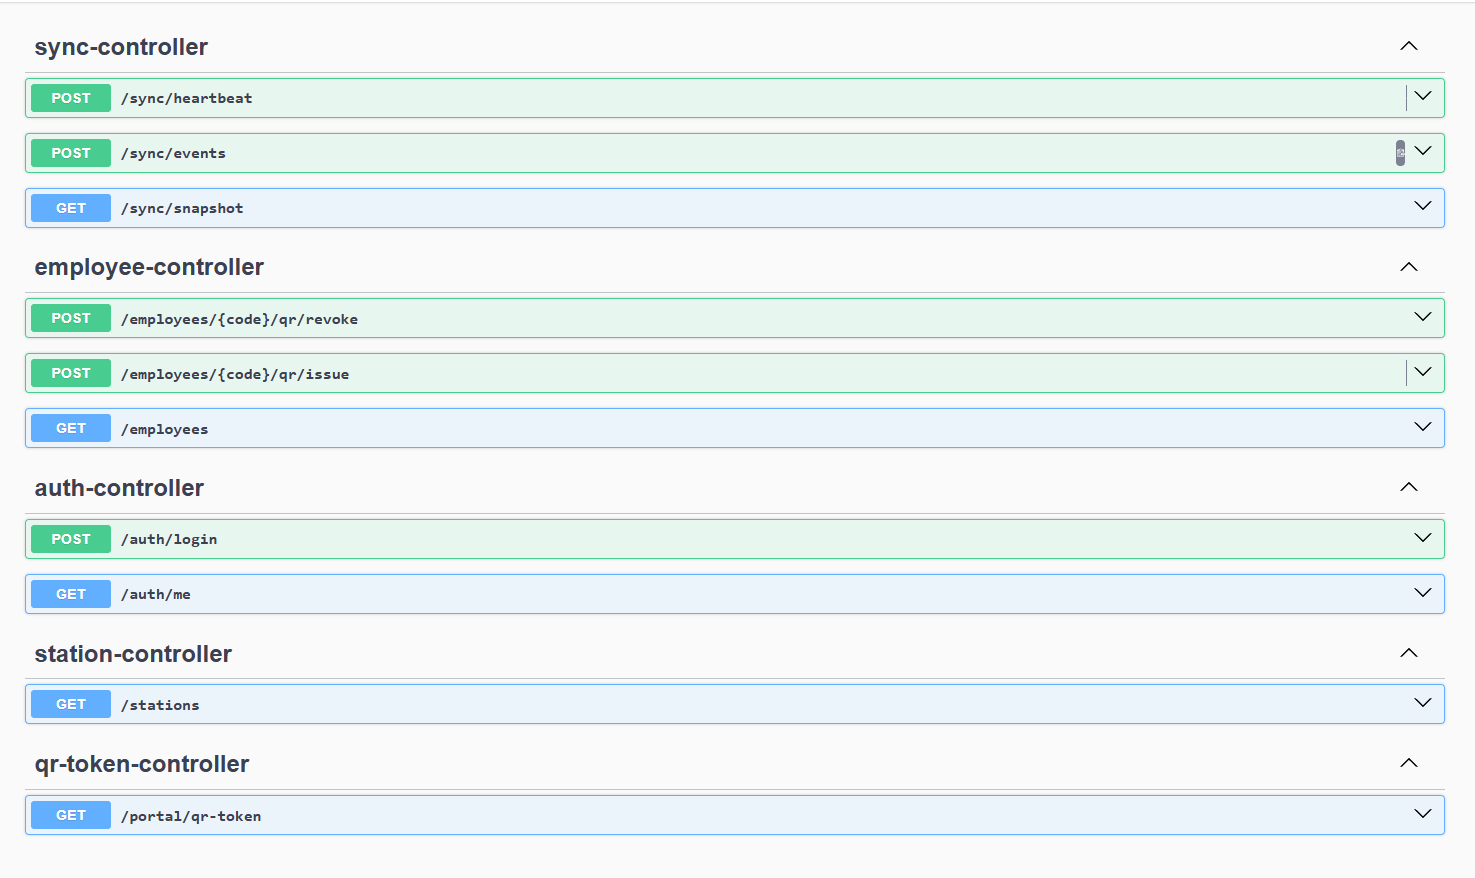
\includegraphics[width=0.92\textwidth]{figures/09_system_implementation/api_swagger_central.png}
    \caption{Giao diện Swagger UI công bố trực tiếp 10 endpoint Central và Sync từ hợp đồng OpenAPI 3.0.3}
    \label{fig:api-swagger-central}
\end{figure}

\subsubsection{Đặc tả chi tiết dữ liệu các API cốt lõi}

Bảng~\ref{tab:core-api-payloads} trình bày cấu trúc dữ liệu đầu vào (request) và đầu ra (response)
của các endpoint trọng yếu nhất trong bốn luồng hoạt động chính của hệ thống.

\small
\begin{longtable}{|>{\raggedright\arraybackslash}p{3.4cm}|>{\raggedright\arraybackslash}p{5.4cm}|>{\raggedright\arraybackslash}p{5.8cm}|}
\caption{Đặc tả dữ liệu đầu vào và đầu ra các API cốt lõi}\label{tab:core-api-payloads}\\
\hline
\textbf{Endpoint} & \textbf{Đầu vào (Request)} & \textbf{Đầu ra thành công (Response)} \\
\hline
\endfirsthead
\hline
\textbf{Endpoint} & \textbf{Đầu vào (Request)} & \textbf{Đầu ra thành công (Response)} \\
\hline
\endhead
\hline
\multicolumn{3}{r}{\textit{Còn tiếp sang trang sau...}} \\
\hline
\endfoot
\hline
\endlastfoot
\texttt{POST /scan} & JSON: \texttt{stationId} (chuỗi \texttt{BD-IN-01}), \texttt{raw} (1--1024 ký tự, chuỗi \texttt{TMC1.<payload>.<sig>}). & \texttt{200 OK}: \texttt{result} (\texttt{ACCEPTED} / \texttt{REJECTED} / \texttt{GATE\_FAILED}), \texttt{reason} (nếu không chấp nhận), \texttt{employeeCode} (chỉ có khi không bị \texttt{REJECTED}), \texttt{direction} (\texttt{IN}/\texttt{OUT}), \texttt{elapsedMs}, \texttt{eventId} (UUID). \\
\hline
\texttt{GET /status} & Không tham số. & \texttt{200 OK}: \texttt{gateId}, \texttt{online} (bool), \texttt{lastSyncAt}, \texttt{outboxDepth}, \texttt{offlineThresholdExceeded} (bool), \texttt{pendingReconcile}, \texttt{turnstiles} (bản đồ \texttt{stationId} $\rightarrow$ \texttt{UP}/\texttt{DOWN}/\texttt{CIRCUIT\_OPEN}). \\
\hline
\texttt{POST /auth/login} & JSON: \texttt{username} (1--32 ký tự, không phân biệt hoa thường), \texttt{password} (1--128 ký tự). & \texttt{200 OK}: \texttt{accessToken} (JWT RS256), \texttt{expiresAt} (+8 giờ), \texttt{role} (\texttt{EMPLOYEE}/\texttt{ADMIN}), \texttt{employeeCode} (chỉ có với \texttt{EMPLOYEE}). \\
\hline
\texttt{GET} \path{/portal/qr-token} & Header \texttt{Authorization: Bearer <JWT>}. Không có tham số. & \texttt{200 OK} (kèm \texttt{Cache-Control: no-store}): \texttt{raw} ($\approx 250$ ký tự), \texttt{expiresAt} (+60 giây), \texttt{refreshAfterSec} (\texttt{30}). \\
\hline
\texttt{POST} \path{/employees/{code}/qr/revoke} & Path \texttt{code} (\texttt{E0012}); JSON: \texttt{reason} (3--200 ký tự sau khi cắt khoảng trắng). & \texttt{200 OK}: đối tượng \texttt{EmployeeView} mới nhất (\texttt{code}, \texttt{fullName}, \texttt{departmentId}, \texttt{departmentName}, \texttt{factoryId}, \texttt{active}, \texttt{credentialId}, \texttt{credentialStatus=REVOKED}, \texttt{issuedAt}). \\
\hline
\texttt{POST /sync/events} & Header \texttt{X-Gate-Key}; JSON \texttt{EventBatch}: \texttt{contractVersion=1}, \texttt{gateId}, \texttt{factoryId}, \texttt{events} (1--200 \texttt{EventEnvelope} gồm \texttt{eventId}, \texttt{type} \texttt{SCAN\_ATTEMPT\_RECORDED} hoặc \texttt{ATTENDANCE\_RECORDED}, \texttt{occurredAt}, \texttt{payload}). & \texttt{200 OK} (\texttt{BatchAck}): \texttt{accepted} (mảng UUID mới lưu), \texttt{duplicates} (mảng UUID đã tồn tại), \texttt{rejected} (mảng \texttt{\{eventId, reason\}} với các lý do \texttt{INVALID\_PAYLOAD}, \texttt{UNKNOWN\_EVENT\_TYPE}, \texttt{UNKNOWN\_STATION}, \texttt{STATION\_NOT\_IN\_FACTORY}). \\
\hline
\texttt{GET /sync/snapshot} & Header \texttt{X-Gate-Key}; Query \texttt{since} (int64, mặc định \texttt{0} lấy toàn phần). & \texttt{200 OK} (\texttt{SnapshotDelta}): \texttt{fromVersion}, \texttt{toVersion}, \texttt{credentials} (không chứa họ tên theo DP-12), \texttt{publicKeys} (Ed25519 SPKI base64), \texttt{stations}, \texttt{settings} (\texttt{offlineThresholdMinutes}). \\
\hline
\texttt{POST /sync/heartbeat} & Header \texttt{X-Gate-Key}; JSON \texttt{Heartbeat}: \texttt{gateId}, \texttt{sentAt}, \texttt{outboxDepth}, \texttt{lastSyncAt}, \texttt{turnstileStatus}. & \texttt{204 No Content}. Central xem Gate là ngoại tuyến nếu quá 30 giây không nhận được heartbeat mới. \\
\hline
\texttt{POST} \path{/turnstiles/{id}/open} & Path \texttt{id} (\texttt{TS-BD-IN-01}); JSON: \texttt{requestId} (UUID chính là \texttt{eventId}). & \texttt{200 OK}: \texttt{requestId}, \texttt{executed=true}, \texttt{duplicate} (bool -- \texttt{true} nếu lệnh đã chạy trước đó), \texttt{at} (thời điểm mở cổng). \\
\hline
\end{longtable}
\normalsize

\subsubsection{Ma trận phân quyền và danh mục mã lỗi chuẩn}

Quyền truy cập API luôn được thực thi tại backend (DP-10); việc ẩn nút trên giao diện chỉ nhằm mục
đích trải nghiệm người dùng. Bảng~\ref{tab:api-auth-matrix} và Bảng~\ref{tab:api-error-codes} tổng
hợp ma trận phân quyền trên Central và danh mục mã lỗi Problem Details dùng chung trên toàn hệ thống.

\begin{table}[H]
\centering
\caption{Ma trận xác thực và phân quyền API phía Central}
\label{tab:api-auth-matrix}
\small
\renewcommand{\arraystretch}{1.25}
\begin{tabularx}{\textwidth}{|>{\raggedright\arraybackslash}X|>{\centering\arraybackslash}p{1.8cm}|>{\centering\arraybackslash}p{2.1cm}|>{\centering\arraybackslash}p{1.8cm}|>{\centering\arraybackslash}p{2.2cm}|}
\hline
\textbf{Nhóm đường dẫn} & \textbf{Công khai} & \textbf{\texttt{EMPLOYEE}} & \textbf{\texttt{ADMIN}} & \textbf{\texttt{X-Gate-Key}} \\
\hline
\texttt{/auth/login}, trang tĩnh, \texttt{/actuator/health}, \texttt{/v3/api-docs} & Cho phép & Cho phép & Cho phép & -- \\
\hline
\texttt{/auth/me} & 401 & Cho phép & Cho phép & -- \\
\hline
\texttt{/portal/qr-token} & 401 & Cho phép & 403 & -- \\
\hline
\texttt{/employees/**}, \texttt{/stations} & 401 & 403 & Cho phép & -- \\
\hline
\texttt{/sync/**} & 401 & 401 & 401 & Cho phép \\
\hline
\end{tabularx}
\end{table}

\begin{table}[H]
\centering
\caption{Danh mục mã lỗi chuẩn (RFC 9457 Problem Details) trên các nhóm API}
\label{tab:api-error-codes}
\small
\renewcommand{\arraystretch}{1.2}
\begin{tabularx}{\textwidth}{|>{\raggedright\arraybackslash}p{4.3cm}|>{\centering\arraybackslash}p{1.2cm}|>{\raggedright\arraybackslash}p{3.0cm}|>{\raggedright\arraybackslash}X|}
\hline
\textbf{Mã \texttt{code}} & \textbf{HTTP} & \textbf{API phát sinh} & \textbf{Ngữ cảnh và xử lý phía client} \\
\hline
\texttt{VALIDATION\_ERROR} & 400 & Mọi API & Thiếu trường bắt buộc, sai kiểu hoặc vượt độ dài; trả kèm danh sách \texttt{errors} theo từng trường. \\
\hline
\texttt{INVALID\_CREDENTIALS} & 401 & \texttt{POST /auth/login} & Sai tài khoản, sai mật khẩu hoặc tài khoản bị khóa (trả cùng một mã lỗi để tránh dò tài khoản). \\
\hline
\texttt{UNAUTHENTICATED} & 401 & Central (JWT) & Thiếu token, token hết hạn hoặc sai chữ ký; client xóa token và quay về màn hình \texttt{AU-01}. \\
\hline
\texttt{FORBIDDEN} & 403 & Central (JWT) & Token hợp lệ nhưng sai vai trò; client hiển thị màn hình \texttt{AU-02}. \\
\hline
\texttt{EMPLOYEE\_NOT\_FOUND} & 404 & \path{/employees/{code}/qr/*} & Mã nhân viên không tồn tại; giao diện tải lại danh sách. \\
\hline
\texttt{CREDENTIAL\_REVOKED}, \texttt{NO\_ACTIVE\_CREDENTIAL}, \texttt{EMPLOYEE\_INACTIVE} & 409 & \path{/portal/qr-token}, \path{/qr/issue}, \path{/qr/revoke} & Xung đột trạng thái nghiệp vụ; Portal chuyển sang \texttt{P-02} và thông báo liên hệ HR. \\
\hline
\texttt{CONCURRENT\_UPDATE} & 409 & \texttt{POST} \path{.../qr/issue} & Hai quản trị viên thao tác đồng thời trên cùng nhân viên; yêu cầu tải lại và thử lại. \\
\hline
\texttt{LOCAL\_STORE\_ERROR} & 500 & Gate \texttt{/scan}, \path{/guard/pending} & Lỗi ghi/đọc SQLite cục bộ; Kiosk báo \textit{``Không xác định -- vui lòng gặp bảo vệ''}. \\
\hline
\texttt{INVALID\_GATE\_KEY}, \texttt{GATE\_MISMATCH}, \texttt{UNKNOWN\_GATE} & 401 / 403 & \texttt{/sync/**} & Sai khóa trạm, sai ánh xạ \texttt{gateId} hoặc trạm chưa đăng ký; Gate giữ nguyên outbox và ghi log lỗi cấu hình. \\
\hline
\texttt{UNSUPPORTED\_}\allowbreak\texttt{CONTRACT\_VERSION}, \texttt{BATCH\_TOO\_LARGE} & 400 & \texttt{POST /sync/events} & Lệch phiên bản hợp đồng (\texttt{$\neq 1$}) hoặc lô vượt quá 200 sự kiện. \\
\hline
\texttt{SIMULATED\_ERROR}, \texttt{SIMULATED\_TIMEOUT} & 500 / 504 & Simulator \texttt{/open} & Lỗi giả lập phần cứng; Gate Agent ánh xạ tương ứng thành \texttt{GATE\_ERROR} và \texttt{GATE\_TIMEOUT}. \\
\hline
\end{tabularx}
\end{table}

Các kịch bản kiểm thử đơn vị, kiểm thử hợp đồng API, kiểm thử tích hợp đầu-cuối (bao gồm kịch bản
mất kết nối WAN, đồng bộ bù outbox, timeout cổng xoay và thu hồi mã QR) cũng như đánh giá hiệu năng
chịu tải giờ giao ca cho toàn bộ các chức năng và endpoint đã hiện thực ở chương này sẽ được trình
bày chi tiết trong Chương 10.
